\def\mytitle{MATRICES USING PYTHON(CIRCLE)}
\def\myauthor{R.Radhika}
\def\contact{r170234@rguktrkv.ac.in}
\def\mymodule{Future Wireless Communication (FWC)}
\documentclass[10pt, a4paper]{article}
\usepackage[a4paper,outer=1.5cm,inner=1.5cm,top=1.75cm,bottom=1.5cm]{geometry}
\twocolumn
\usepackage{graphicx}
\graphicspath{{./images/}}
\usepackage[colorlinks,linkcolor={black},citecolor={blue!80!black},urlcolor={blue!80!black}]{hyperref}
\usepackage[parfill]{parskip}
\usepackage{lmodern}
\usepackage{tikz}
	\usepackage{physics}
%\documentclass[tikz, border=2mm]{standalone}
%\usepackage{karnaugh-map}
%\documentclass{article}
\usepackage{tabularx}
%\usepackage{circuitikz}
\usepackage{enumitem}
\usetikzlibrary{calc}
\usepackage{amsmath}
\usepackage{amssymb}
\renewcommand*\familydefault{\sfdefault}
\usepackage{watermark}
\usepackage{lipsum}
\usepackage{xcolor}
\usepackage{listings}
\usepackage{float}
\usepackage{titlesec}
\providecommand{\mtx}[1]{\mathbf{#1}}
\titlespacing{\subsection}{1pt}{\parskip}{3pt}
\titlespacing{\subsubsection}{0pt}{\parskip}{-\parskip}
\titlespacing{\paragraph}{0pt}{\parskip}{\parskip}
\newcommand{\figuremacro}[5]{
    \begin{figure}[#1]
        \centering
        \includegraphics[width=#5\columnwidth]{#2}
        \caption[#3]{\textbf{#3}#4}
        \label{fig:#2}
    \end{figure}
}

\newcommand{\myvec}[1]{\ensuremath{\begin{pmatrix}#1\end{pmatrix}}}
\let\vec\mathbf
\lstset{
frame=single, 
breaklines=true,
columns=fullflexible
}

\title{\mytitle}
\author{\myauthor\hspace{1em}\\\contact\\FWC22066\hspace{6.5em}IITH\hspace{0.5em}\mymodule\hspace{6em}Assignment}
\begin{document}
	\maketitle
	\tableofcontents
   \section{Problem}
   The centre of the circle passing through (0,0)and (1,0) and touching the circle
   $x^2+y^2=9$
\section{Construction}
  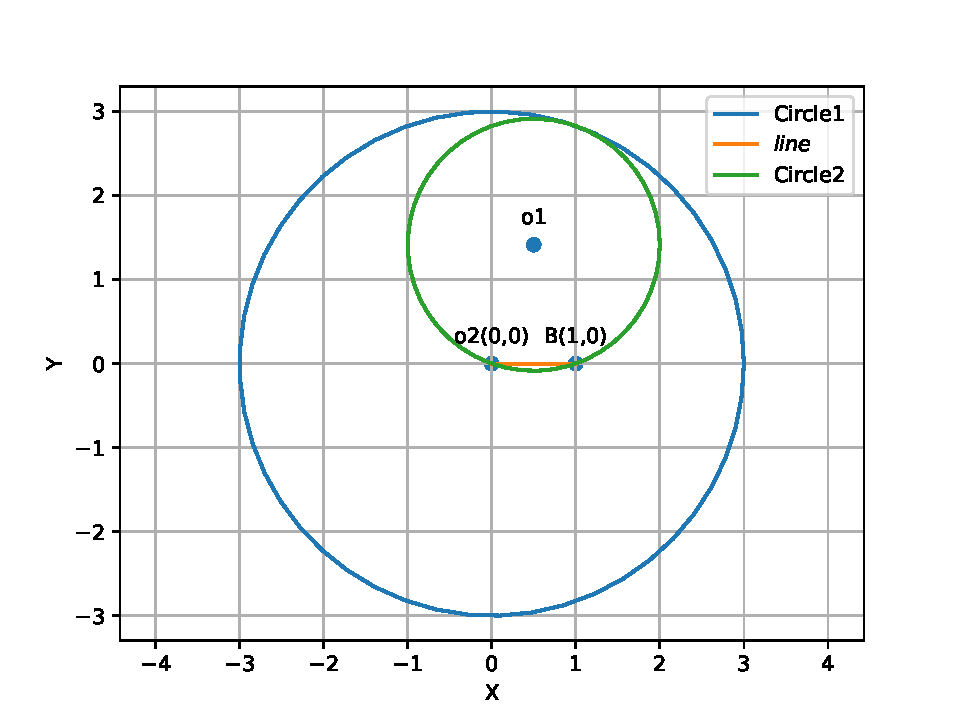
\includegraphics[scale=0.47]{figure1.pdf}
  	\begin{center}
  Figure of construction
  	\end{center}
  \section{Solution}
The standard circle equation\\
\begin{align}
\vec{x}^{\top}\vec{V}\vec{x}+2\vec{u}^{\top}\vec{x}+f=0
\end{align}
Given Circle equation : $x^2+y^2=9$\\
The given circle  can be expressed as conics with parameters
\begin{align}
\vec{x}^{\top}\myvec{1&0\\0&1}\vec{x}+2\myvec{0&0}\vec{x}+f_2=0
\end{align}
\begin{align}
	\vec{V_1} &= \vec{I}, \vec{u_2} = \myvec{0\\0}, f_2 = -9
	\end{align}
	Radius and Centre are
\begin{align}
r_2=\sqrt{{\vec{u_2}^{\top}\vec{u_2}}-f_2 }\\
{r_2}=3
\end{align}
The given circle  can be expressed as conics with parameters
For finding center $\vec{u_1}$
\begin{align}
\vec{x}^{\top}\vec{V}\vec{x}+2\vec{u_1}^{\top}\vec{x}+f_1=0
\end{align}
\begin{align}
    \vec{A}^{\top}\vec{A}+2\vec{u_1}^{\top}\vec{A}+f_1=0
    \end{align}
\begin{align}
\vec{B}^{\top}\vec{B}+2\vec{u_1}^{\top}\vec{B}+f_1=0
\end{align}
\begin{align}
\vec{V} &= \myvec{1 & 0\\0 & 1},\vec{A}= \myvec{0\\0} ,\vec{B}= \myvec{1\\0}
\end{align}
when  substitute $\vec{A},\vec{B}$ in eq 6and 7\\
$f_1=0$,\\
by eq 7
\begin{align}
1+2\vec{u_1}^{\top}\myvec{1\\0}+f_1=0
\end{align}
\begin{align}
1+2\vec{u_1}^{\top}\vec{e_1}=0
\end{align}
\begin{align}
\vec{u_1}^{\top}\vec{e_1}=-1/2
\end{align}
\begin{align}
\vec{u_1}=\myvec{x\\y}
\end{align}
substitute in eq-11
\begin{align}
\myvec{x&y}\myvec{1\\0}=-1/2
\end{align}
\begin{align}
x=-1/2
\end{align}
substitute x in eq-13
\begin{align}
\vec{u_1}=\myvec{-1/2\\y}
\end{align}
\begin{align}
\norm{\vec{u_1}-\vec{u_2}}=(r_1-r_2)^2
\end{align}
\begin{align}
r_1=\frac{r_2}{2}
\end{align}
\begin{align}
\norm{\vec{u_1}}^2=r_1^2
\end{align}
\begin{align}
\norm{\vec{u_1}}^2=(r_2/2)^2
\end{align}
by using eq-15\\
\begin{align}
\norm{\vec{u_1}}^2=1/4+y^2=\frac{r_2^2}{4}
\end{align}
\begin{align}
y=\pm\sqrt{\frac{r_2^2}{4}-\frac{1}{4}}
\end{align}
yielding,
\begin{align}
y=\pm\sqrt{2}
\end{align}
substituting y in eq-15\\
\begin{align}
\vec{u_1}=\myvec{-1/2\\-\sqrt{2}}
\end{align}
\begin{align}
\vec{o_1}=\vec{-u_1}
\end{align}
\begin{align}
r_1=\sqrt{{\vec{u_1}^{\top}\vec{u_1}}-f_1 }
\end{align}
\begin{align}
{r_1}=3/2
\end{align}

The input parameters for this construction are
\begin{center}
\begin{tabular}{|c|c|c||c|}
	\hline
	\textbf{Symbol}&\textbf{Value}&\textbf{Description}\\
	\hline
	$\vec{A}$ &\myvec{0\\0}& Centre1,point p1\\
	\hline
    $\vec{B}$ &\myvec{1\\0}&point2\\
	\hline
    $\vec{o_2}$&\myvec{-1/2\\-\sqrt{2}}&center2\\
	\hline
	$\vec{R}$&\myvec{1.5}& Radius2\\
	\hline
\end{tabular}

Below python code realizes the above construction 
\begin{table}[h]
    \centering
    \begin{tabular}{|c|}
    \hline \\
         https://github.com/Radhikarkv/fwcproject.git  \\
         \\
\hline
    \end{tabular}
\end{table}
\end{center}
\end{document}
